\documentclass[11pt,a4paper]{article}
\usepackage[margin=2.5cm]{geometry}
\usepackage{amsmath,amssymb}
\usepackage{booktabs}
\usepackage{graphicx}
\usepackage{xcolor}
\emergencystretch=3em
\usepackage[colorlinks=true,linkcolor=blue!60!black,citecolor=blue!60!black,urlcolor=blue!60!black]{hyperref}
\graphicspath{{./}{../}}

\newcommand{\mcatnlo}{\textsc{MC@NLO}}
\newcommand{\mg}{\textsc{MadGraph7}}
\newcommand{\rS}{r_{\mathrm S}}
\newcommand{\rH}{r_{\mathrm H}}
\newcommand{\Neff}{N_{\mathrm{eff}}}
\newcommand{\dd}{\mathrm{d}}
\newcommand{\code}[1]{\texttt{#1}}

\title{Folding the radiation phase space in \mcatnlo:\\
the lattice, the cubic map, and the sum over FKS sets}
\author{O.~Mattelaer}
\date{October 2026}

\begin{document}
\maketitle

\begin{abstract}
In \mcatnlo{} event generation, every unweighted S event carries the integral of the
subtraction terms over the variables of the extra emission, $(\xi_i,y_{ij},\phi_i)$, estimated
by Monte Carlo at a fixed underlying Born configuration. A negative estimate produces a
negative-weight event even when the exact integral is positive. ``Folding'' reduces these
negative weights by evaluating the integrand at several points in the radiation variables for each Born
phase-space point. We describe three ways of choosing and combining these points:
(i)~the equally spaced, randomly shifted lattice used today,
(ii)~the same lattice after the cubic change of variables $s=t^2(3-2t)$, and
(iii)~the sum of the S-event contributions over all sets of FKS configurations instead of
one set picked at random. All three are exact in the limit of infinite statistics: they change the size of the
fluctuations, never the expectation. We explain why a deterministic Simpson rule is
\emph{not} acceptable, why the cubic map gives an error falling like $n^{-2}$ instead of
$n^{-1}$ (and not like Simpson's $n^{-4}$), and why summing over FKS sets can only lower the
fraction of negative S weight. We then measure the negative-weight fractions and the CPU cost
for $pp\to t\bar t$, $pp\to e^+e^-j$, $e^+e^-\to b\bar b b\bar b$ and $pp\to Zjj$ at NLO in
QCD. The combination of the cubic map and the sum over FKS sets with $2\times2\times1$
folding matches, or beats, today's $8\times4\times1$ folding at 3.5 to 7 times less CPU per
effective event. The remaining negative weights are dominated by H events, which no
folding can affect.
\end{abstract}

\tableofcontents

%======================================================================
\section{Negative weights in \mcatnlo{} and what folding does}
\label{sec:intro}

In the \mcatnlo{} method~\cite{Frixione:2002ik}, as implemented with FKS
subtraction~\cite{Frixione:1995ms,Frederix:2009yq} in
\textsc{MadGraph5\_aMC@NLO}~\cite{Alwall:2014hca} and \mg, the cross section is written as
the sum of two kinds of events:
\begin{itemize}
\item \textbf{H events}, with the kinematics of the real emission, weighted by the real-emission
matrix element minus the \mcatnlo{} counterterm, $R-\mathrm{MC}$;
\item \textbf{S events}, with Born kinematics, weighted by the Born, the virtual and the
integrated counterterms, plus the integral over the radiation variables of the \mcatnlo{}
counterterm minus the FKS counterterms.
\end{itemize}
After unweighting, each event has weight $\pm w$. If a fraction $r$ of the events is negative,
the statistical power of a sample of $N$ events is that of
\begin{equation}
  \Neff = N(1-2r)^2
\end{equation}
positive events. With $r=0.3$ one needs six times more events than without negative weights.
We use $\rS$ and $\rH$ for the negative fractions of the S and H events separately.

\paragraph{The S-event weight at a fixed Born point.}
Let $\Phi_B$ be the Born variables and $u=(u_\xi,u_y,u_\phi)\in[0,1]^3$ the radiation
variables, in the flat coordinates of the adaptive (vegas-like) grids of the MINT
integrator~\cite{Nason:2007vt}. For a given $\Phi_B$, the S-event weight is
\begin{equation}
  S(\Phi_B) = \int_{[0,1]^3}\dd^3u\;\Big[\,\mathcal B(\Phi_B)\,J(u)
                               + \sum_{k=1}^{N_{\mathrm{sets}}} C_k(\Phi_B,u)\Big] ,
  \label{eq:S}
\end{equation}
where:
\begin{itemize}
\item $\mathcal B$ collects the $n$-body terms: Born, virtual (or its average in the
``virt-trick''), and the analytically integrated soft and collinear terms;
\item $J(u)$ is the product of the grid and FKS Jacobians of the radiation variables, with
$\int J=1$;
\item $C_k$ is the sum, over the FKS configurations of set $k$, of all the $(n{+}1)$-body
contributions that go into S events: the S part of the \mcatnlo{} counterterm, the soft,
collinear and soft-collinear FKS counterterms, and the collinear remnants.
\end{itemize}
A set of FKS configurations groups one configuration with a soft singularity and the
configurations without one that are attached to it. There are 3 to 4 sets for the processes
studied here.

The exact $S(\Phi_B)$ is, for most Born points, positive. But the code does not have it: it
has a Monte Carlo estimate $\hat S(\Phi_B)$, and an S event is negative whenever $\hat S<0$.
Two sources of fluctuation enter $\hat S$:
\begin{enumerate}
\item the estimate of the integral over $u$, from one or a few points in the radiation variables;
\item the choice of a single set $k$ by Monte Carlo (the default ``\code{sum=3}'' mode).
\end{enumerate}

\paragraph{What folding is.}
With folding $n_\xi\times n_y\times n_\phi$ (run-card entry \code{folding}), the integrand is
evaluated at $n=n_\xi n_y n_\phi$ images of the same Born point. All the S-event
contributions of these images are added into a single S event before its sign is taken.
The H events of the images stay separate events: they have different kinematics. Folding
therefore acts only on the S events, and only on the first source of fluctuation above. The
choice of FKS set is made once per Born point, before the images are generated, and is
shared by all of them.

\paragraph{Exactness.}
A method is acceptable only if it is exact on average: for any distribution, the average
over events must converge to the right result as the statistics grow. Faster convergence
or fewer negative weights may only change the size of the fluctuations. This rules out
any deterministic rule whose error does not average away (section~\ref{sec:simpson}).

%======================================================================
\section{Mode 1: the randomly shifted lattice (today's folding)}
\label{sec:lattice}

MINT~\cite{Nason:2007vt} splits each folded dimension, of $N_{\mathrm{int}}$ grid
intervals, into $n$ groups of $N_{\mathrm{int}}/n$ adjacent intervals. It picks a cell and a
position inside it in the first group, and then takes the same relative position in each of
the $n$ groups. In the flat coordinate $t\in[0,1)$ of the grid, the images are
\begin{equation}
  t_k = \frac{U+k-1}{n},\qquad k=1,\dots,n,\qquad U\sim\mathcal U[0,1),
  \label{eq:lattice}
\end{equation}
and they all have weight $1/n$. The vegas map $x(t)$ and its Jacobian $x'(t)$ then turn
$t_k$ into the physical variable. Writing $f(t)$ for the integrand in the flat coordinate
(Jacobian included), the estimate is
\begin{equation}
  \hat I_{\mathrm{lat}} = \frac1n\sum_{k=1}^n f(t_k).
\end{equation}
This is a rectangle rule with a random shift, a Cranley--Patterson rotation~\cite{Cranley:1976}. In three
dimensions it is the product of three such rules.

\paragraph{Exact on average.}
Each $t_k$ is uniformly distributed on $[0,1)$, so $\mathbb E[f(t_k)]=\int_0^1 f$ for
every $k$, and $\mathbb E[\hat I_{\mathrm{lat}}]=\int_0^1 f$ for any $f$.

\paragraph{Error.}
Extend $f$ periodically. For a smooth $f$ the Euler--Maclaurin formula gives, for one shift $U$,
\begin{equation}
  \hat I_{\mathrm{lat}}-\int_0^1 f = -\frac{f(1)-f(0)}{n}\Big(U-\tfrac12\Big)+\mathcal O(n^{-2}).
  \label{eq:EMlattice}
\end{equation}
The leading term comes from the jump of the periodic extension at $t=0\equiv1$. Its RMS over $U$ is
$|f(1)-f(0)|/(\sqrt{12}\,n)$: the lattice is a first-order rule unless the integrand happens
to take the same value at both ends. In the radiation variables it never does: the
integrand is large near the soft ($\xi\to0$) and collinear ($y\to1$) endpoints, where the
grid is also densest.

\paragraph{The $n$-body term as a control variate.}
In equation~\eqref{eq:S} the $n$-body term enters with the density $J(u)$, the product of the grid
and FKS Jacobians. The grid adapts to $|f|$, so $J$ is large precisely where the
counterterms $C_k$ are large and negative. Folding evaluates $\mathcal B J(u_k)$ at each image,
and the $n$-body term then partly cancels the counterterms point by point. Replacing
$\mathcal B J(u_k)$ by its exact integral $\mathcal B$ (which would remove its fluctuation)
makes the negative fraction much \emph{worse}: for $t\bar t$ at $8\times4\times1$, $\rS$
rises from $0.0006$ to $0.04$ in our dumps. The non-flat $n$-body density is a free control
variate, and every mode below keeps it.

%======================================================================
\section{Why not a (deterministic) Simpson rule}
\label{sec:simpson}

The composite Simpson rule on $[0,1]$, with nodes $j/m$ and weights $(1,4,2,4,\dots,4,1)/(3m)$,
has an error $\mathcal O(m^{-4})$ for a smooth integrand. Two properties make it unusable here:
\begin{enumerate}
\item \textbf{It is not exact on average.} The nodes are fixed, so its error at each Born
point has a definite sign. The error does not average away over Born points: it is a bias
of the cross section and of every distribution.
\item \textbf{The integrand is not smooth.} In the flat grid coordinates the S-event
integrand has integrable endpoint singularities (soft and collinear limits), steps (the
shower dead zones of the \mcatnlo{} counterterm, the cuts $\xi<\xi_{\mathrm{cut}}$ and
$y>1-\delta$), and steep PDF ratios in the collinear remnants. Simpson's error bound does
not apply.
\end{enumerate}
The endpoints also cannot be evaluated: at $\xi=0$ or $y=1$ the counterterm prefactors are
singular. They have to be displaced slightly, by $10^{-7}$ in our tests.

Table~\ref{tab:simpson} shows the bias of the average S weight, measured on the same Born
points against a randomised reference rule with 256 points (section~\ref{sec:dumps}). It
is $\mathcal O(10\%)$ and shrinks only slowly with $m$. A deterministic Simpson rule is
therefore excluded. Note that the question is not the precision per Born point (it only
needs to be right on average) but this bias of the average.

\begin{table}[t]
\centering
\begin{tabular}{lccc}
\toprule
rule (intervals in $\xi\times y$) & points & bias of $\langle S\rangle$, $t\bar t$ & bias of $\langle S\rangle$, $e^+e^-j$ \\
\midrule
Simpson $2\times2$ & 9  & $-12.6\%$ & $+36\%$ \\
Simpson $4\times4$ & 25 & $-11.2\%$ & $+22\%$ \\
Simpson $8\times8$ & 81 & $-6.7\%$  & -- \\
\bottomrule
\end{tabular}
\caption{Bias of the average S-event weight with a deterministic composite Simpson rule in the radiation variables.}
\label{tab:simpson}
\end{table}

%======================================================================
\section{Mode 2: the cubic map}
\label{sec:cubic}

\subsection{Definition}
To gain the accuracy of a higher-order rule while staying exact on average, keep the random
lattice of equation~\eqref{eq:lattice} but change the variable first. With any increasing bijection
$\varphi:[0,1]\to[0,1]$,
\begin{equation}
  \int_0^1 f(s)\,\dd s=\int_0^1 f(\varphi(t))\,\varphi'(t)\,\dd t
  \quad\Longrightarrow\quad
  \hat I_\varphi=\frac1n\sum_{k=1}^n f\big(\varphi(t_k)\big)\,\varphi'(t_k).
  \label{eq:transformed}
\end{equation}
\code{FoldCubic} uses
\begin{equation}
  \varphi(t)=t^2(3-2t),\qquad \varphi'(t)=6t(1-t),
  \label{eq:cubic}
\end{equation}
which is applied to $\xi_i$ and $y_{ij}$ whenever that variable is folded ($n>1$). The image $k$
is placed at $s_k=\varphi(t_k)$ in the flat grid coordinate and carries the weight
$\varphi'(t_k)/n$ instead of $1/n$. Nothing else changes: the grid, the upper bounding envelope
(indexed by the shift $U$, as before), and the treatment of the H events.

\subsection{It is not a spline: the case of two points}
The name ``cubic'' refers to the polynomial $\varphi$ of equation~\eqref{eq:cubic}, the ``smoothstep'',
and not to an interpolation. Nothing is fitted through the points, so the method does not
need four, or even two, points. Figure~\ref{fig:cubicmap} shows what happens with $n=2$
images and the shift $U=0.3$:
\begin{itemize}
\item \textbf{Lattice:} $t_1=0.15$ and $t_2=0.65$, each with weight $1/2$. The images are at
$s_1=0.15$ and $s_2=0.65$.
\item \textbf{Cubic:} the same $t_1,t_2$ are mapped to $s_1=\varphi(0.15)=0.061$ and
$s_2=\varphi(0.65)=0.718$. Their weights are $\varphi'(0.15)/2=0.383$ and $\varphi'(0.65)/2=0.683$.
\end{itemize}
For one Born point the two weights do not sum to 1. They sum to $1$ only on average over
$U$:
\begin{equation}
  \mathbb E_U\Big[\tfrac12\varphi'(\tfrac U2)+\tfrac12\varphi'(\tfrac{U+1}2)\Big]
  =\int_0^1\varphi'(t)\,\dd t=1 .
\end{equation}
More generally, for any integrand,
\begin{equation}
  \mathbb E_U\big[\hat I_\varphi\big]
  =\frac1n\sum_{k}\int_0^1\!\dd U\, f\big(\varphi(\tfrac{U+k-1}{n})\big)\,\varphi'(\tfrac{U+k-1}{n})
  =\int_0^1 f(\varphi(t))\varphi'(t)\,\dd t=\int_0^1 f(s)\,\dd s ,
\end{equation}
for every $n$, including $n=1$. The cubic map is thus an \emph{importance-sampling-like
reweighting combined with a random shift}. The images move toward the endpoints, where the
integrand is large, and carry smaller weights there.

\begin{figure}[t]
\centering
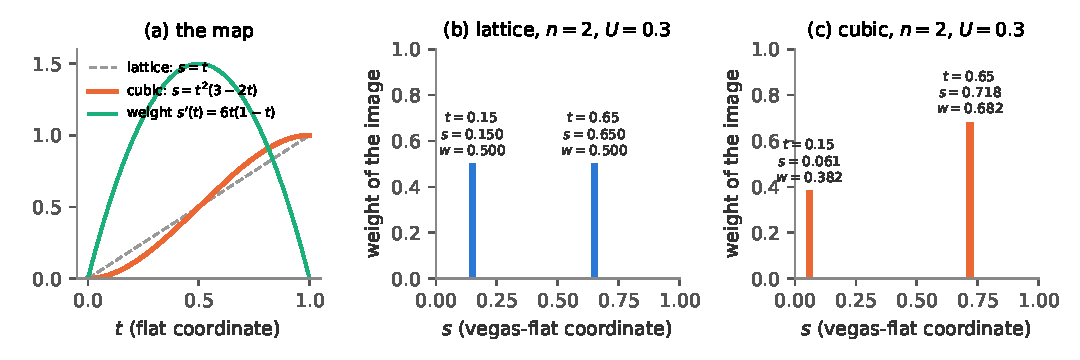
\includegraphics[width=\textwidth]{fig_cubic_map.pdf}
\caption{(a) The cubic map $s=\varphi(t)$ and its weight $\varphi'(t)$. (b, c) Positions in
the flat grid coordinate and weights of the two images of one Born point, for folding $n=2$
and shift $U=0.3$, with the lattice and with the cubic map.}
\label{fig:cubicmap}
\end{figure}

\subsection{Order of the rule}
Equation~\eqref{eq:transformed} is the lattice rule applied to $g(t)=f(\varphi(t))\varphi'(t)$. Since
$\varphi'(0)=\varphi'(1)=0$, $g$ vanishes at both ends. Its periodic extension is therefore
continuous, and the $\mathcal O(n^{-1})$ term of equation~\eqref{eq:EMlattice}, which came from the jump
$f(1)-f(0)$, is gone. The first derivative,
\begin{equation}
  g'(0)=6f(0),\qquad g'(1)=-6f(1),
\end{equation}
still jumps at the wrap-around, so the error is $\mathcal O(n^{-2})$ for a smooth $f$: a
\textbf{second-order rule}, like the trapezoid rule. It is \emph{not} of Simpson's order
$n^{-4}$. (We called it ``Simpson-order'' in a first version of the code comments, which
was wrong. Making $g'$ continuous too requires the quintic map
$\varphi=t^3(10-15t+6t^2)$, which gives $n^{-3}$; each further order needs a higher-degree
polynomial, as in Sidi-type transformations~\cite{Sidi:1993}.)

Figure~\ref{fig:convergence} confirms the orders on three test functions:
\begin{itemize}
\item \textbf{Smooth integrand} ($e^x$): the RMS error falls like $n^{-1}$ (lattice),
$n^{-2}$ (cubic) and $n^{-3}$ (quintic).
\item \textbf{Integrable endpoint singularity} ($x^{-1/2}$, the shape of a soft or
collinear limit after the FKS map): the lattice converges only like $n^{-1/2}$. The node
closest to the endpoint samples a heavy tail. With the cubic map
$g(t)\simeq(3t^2)^{-1/2}\,6t$ stays bounded near $t=0$ and the error falls like $n^{-1}$.
This is the most relevant gain for our integrands.
\item \textbf{Step} ($\theta(x-0.3)$): every map is back to $n^{-1}$, with a similar constant.
A step at a random position cannot be integrated better than this by any rule that does not
know where it is.
\end{itemize}

\begin{figure}[t]
\centering
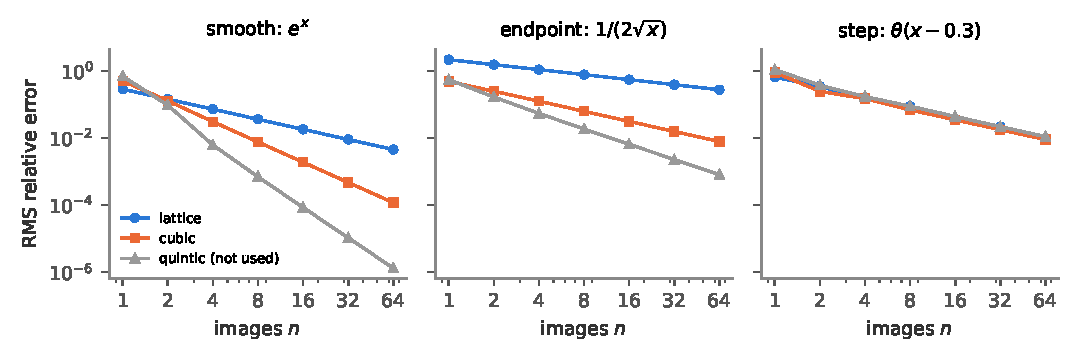
\includegraphics[width=\textwidth]{fig_convergence.pdf}
\caption{RMS relative error of the randomly shifted rule with $n$ images, for the lattice,
the cubic map and (for comparison) the quintic map, on a smooth integrand, an integrable
endpoint singularity and a step. $2\times10^4$ random shifts.}
\label{fig:convergence}
\end{figure}

\paragraph{Practical consequences.}
\begin{enumerate}
\item \textbf{With one image the cubic map only adds noise}: the weight $6U(1-U)$
fluctuates and nothing compensates it. The code therefore applies it only to a folded
variable ($n>1$), and a $1\times1\times1$ run is unchanged.
\item \textbf{For the S-event integrand, the gain is a constant factor rather than a
better order}, because the integrand contains steps (dead zones and cuts). The dumps of
section~\ref{sec:dumps} show convergence close to $n^{-1/2}$ in every rule, the cubic map
being worth about 2 to 4 times fewer points than the lattice.
\item \textbf{The H events are not affected in their sign.} Each image still gives its own
H event, with weight $\varphi'(t_k)/n\le 1.5/n$.
\end{enumerate}

%======================================================================
\section{Mode 3: summing the S events over FKS sets}
\label{sec:sumsets}

\subsection{The Monte Carlo over FKS sets}
In the default mode (\code{sum=3}), for each Born point one set $k$ of FKS configurations is
picked with probability $p_k$, adapted during the integration. With $\alpha_k=1/N_{\mathrm{sets}}$
the S-event estimate is then
\begin{equation}
  \hat S_k = \frac{\alpha_k\,\mathcal B\,\hat J + \hat C_k}{p_k},
  \qquad \mathbb E_k\big[\hat S_k\big]=\sum_k p_k\hat S_k=\mathcal B\hat J+\sum_k \hat C_k ,
  \label{eq:MCsets}
\end{equation}
where hats denote the folded estimates over the images. The weight of the $n$-body term,
$1/(N_{\mathrm{sets}}\,p_k)$, and that of the counterterms of the picked set, $1/p_k$,
fluctuate with the choice of set. The S event of a given Born point can therefore be
negative because the picked set happens to have large negative counterterms, even when
the sum over all sets is positive.

\subsection{Summing the S contributions}
With \code{FoldSumSets}, every image loops over \emph{all} sets and adds the S-event
contributions of each set with weight 1:
\begin{equation}
  \hat S_\Sigma = \mathcal B\,\hat J+\sum_k \hat C_k .
\end{equation}
The H-event contributions, and with them the evaluation of the real-emission matrix element,
still come from the set picked by Monte Carlo, divided by its probability:
\begin{equation}
  \hat H = \frac{\hat H_k}{p_k}\quad\text{with probability } p_k .
\end{equation}
Both pieces are exact on average, so their sum is. The extra cost is the evaluation, for the
sets that are not picked, of the S part of each image: kinematics, \mcatnlo{} and FKS
counterterms, colour-linked Borns and PDFs. The real-emission matrix element is not
evaluated more often.

\subsection{It can only lower the S-event negative fraction}
At a given Born point and set of images, $\hat S_\Sigma=\sum_k p_k\hat S_k$, so by the triangle
inequality
\begin{equation}
  |\hat S_\Sigma| \;\le\; \sum_k p_k\,|\hat S_k| = \mathbb E_k\big[|\hat S_k|\big],
\end{equation}
while the signed weights have the same expectation. After unweighting, the negative fraction
of the S events is
$\rS=\big(\langle|\hat S|\rangle-\langle\hat S\rangle\big)/\big(2\langle|\hat S|\rangle\big)$.
Summing lowers $\langle|\hat S|\rangle$ at fixed $\langle\hat S\rangle$, so $\rS$ can only
decrease, point by point. The same inequality holds whenever an estimate is replaced by the
average of several independent copies of itself. It does \emph{not} say that any rule with
more images is better than any rule with fewer: a $4\times4$ lattice is not the average of
independent $2\times2$ lattices. Neither does it cover the events that the folding does not
touch (section~\ref{sec:floor}). The gain is large when the sets have counterterms of different
sizes, which is the case as soon as there are initial-state and final-state collinear
singularities (e.g.\ $pp\to e^+e^-j$). It is small when one set dominates.

\subsection{Implementation notes}
\begin{itemize}
\item The H-type contributions (real emission, and counterterms with $(n{+}1)$-body kinematics)
are dropped in \code{add\_wgt} for the sets that are not picked, and rescaled by $1/p_k$ for
the picked one.
\item The Born momenta computed for different sets differ in their last bits. The cache of
the Born amplitudes is therefore asked to re-check its momenta and couplings between sets
and before the event is written. With the $\alpha_s$ rescaling of the cached Born
(``gscale'', PR~\#305, after MadVfold~\cite{Valassi:2026pgd}), this check is cheap.
\item \textbf{Open question.} The S-event shower starting scale is assigned from one of the
contributions, picked by weight. With summed sets this choice runs over all sets instead of
the picked one. This is a matching-level choice that has not been validated after the shower.
\end{itemize}

%======================================================================
\section{Studies at a fixed Born point}
\label{sec:dumps}

To separate the error of the integral over the radiation variables from the other
fluctuations, a study-only mode of the code
evaluated several rules on the \emph{same} Born points: each rule with several independent
shifts, and optionally with the FKS set forced. We used about $10^4$ Born points per
process, in the two dominant channels of $t\bar t$ (gg, $u\bar u$) and of $e^+e^-j$ ($ug$,
$u\bar u$).

\paragraph{Precision per Born point.}
Table~\ref{tab:fixedset} gives the median relative error of the S weight of one FKS set at one
Born point, against a 256-point cubic reference. Two independent 256-point estimates for
$e^+e^-j$ already differ by a median of 18--21\%. The convergence is close to $n^{-1/2}$ for
every rule. Reaching 1\% per Born point would need of order $2\times10^3$ points for
$t\bar t$ and more than $10^4$ for $e^+e^-j$. As noted in the introduction, this precision is
not needed: only the sign matters, and the average is exact anyway.

\begin{table}[t]
\centering
\begin{tabular}{lccc}
\toprule
rule & points & $t\bar t$ & $e^+e^-j$\\
\midrule
lattice $2\times2$ & 4  & 21\% & 46\% \\
lattice $8\times4$ & 32 & 12\% & 29\% \\
cubic $4\times4$   & 16 & 10\% & 27\% \\
cubic $8\times4$   & 32 & 8\%  & 25\% \\
rank-1 lattice (cubic), $N=21$ & 21 & 7\% & 26\% \\
\bottomrule
\end{tabular}
\caption{Median relative error of the S weight of one FKS set at one Born point.}
\label{tab:fixedset}
\end{table}

\paragraph{Negative S fraction versus rule.}
Table~\ref{tab:dumpr} shows $\rS$ for several rules, with the FKS set picked by Monte Carlo
(today) or summed. The numbers come from MINT1-type weights in two channels. They
are a relative comparison only, about $0.03$ below the full runs of
section~\ref{sec:runs}. We draw three conclusions:
\begin{itemize}
\item For $t\bar t$, the cubic $2\times2$ rule already has 5 times fewer S negatives than the
$2\times2$ lattice.
\item For $e^+e^-j$, $\rS$ reaches a floor of about $0.07$ even with 256 points when one set
is picked, and about $0.03$ when the sets are summed. The choice of FKS set, not the
quadrature, limits the S events.
\item Quasi-random rank-1 (Fibonacci) lattices and the other maps we tried (tent, quintic,
$t-\sin(2\pi t)/2\pi$) do not beat the cubic map. They were removed from the code.
\end{itemize}

\begin{table}[t]
\centering
\begin{tabular}{lcccc}
\toprule
rule & points & $t\bar t$, $\rS$ (MC sets) & $e^+e^-j$, $\rS$ (MC sets) & $e^+e^-j$, $\rS$ (summed sets)\\
\midrule
lattice $1\times1$ & 1 & 0.062 & 0.249 & 0.175 \\
lattice $4\times4$ & 16 & 0.0013 & 0.120 & 0.067 \\
lattice $8\times4$ & 32 & 0.0006 & 0.094 & 0.040 \\
cubic $2\times2$ & 4 & 0.0016 & 0.138 & 0.058 \\
cubic $4\times4$ & 16 & 0.0003 & 0.084 & 0.031 \\
cubic $16\times16$ & 256 & 0.0002 & 0.073 & 0.030 \\
\bottomrule
\end{tabular}
\caption{S-event negative fraction at fixed Born points ($\sim10^4$ points; bootstrap errors
$\pm0.01$ for $e^+e^-j$).}
\label{tab:dumpr}
\end{table}

%======================================================================
\section{Results of complete runs}
\label{sec:runs}

\subsection{Setup}
We ran complete \mcatnlo{} event generations (no shower) at NLO in QCD for four processes:
\begin{itemize}
\item $pp\to t\bar t$ (\code{loop\_sm-no\_b\_mass}, 13~TeV, 20k events);
\item $pp\to e^+e^-j$ (same model, 10k events);
\item $e^+e^-\to b\bar b b\bar b$ (default \code{sm}, $m_b=4.7$~GeV, $\sqrt s=1$~TeV, 10k events);
\item $pp\to Zjj$ (13~TeV, NNPDF4.0 $n_f=4$, anti-$k_T$ $R=0.4$, $p_{T,j}>30$~GeV, 10k events
with the accuracy target of 2000 events).
\end{itemize}
All runs use seed 21. The negative fractions are counted from the event signs; the CPU is
the MINT1+MINT2 time summed over jobs.

Timing on a shared desktop turned out to be fragile: a virus-scanner load spike inflated the
process CPU time by up to $1.7$--$2\times$. All CPU numbers below come from runs at normal load:
\begin{itemize}
\item $t\bar t$ and $e^+e^-j$ re-run consecutively at normal load;
\item $e^+e^-\to b\bar b b\bar b$ with the code before and after PR~\#305 running side by side;
\item $Zjj$ on a cluster node, also side by side.
\end{itemize}
They are good to about $\pm10$--$20\%$. Same-seed re-runs reproduce $\sigma$ and $r$ exactly.

\subsection{Tables and plots}
Tables~\ref{tab:tt}--\ref{tab:zjj} list, for each variant, the negative fractions, the CPU
per event and the CPU per effective event. Figures~\ref{fig:tt_eej}--\ref{fig:zjj} show
$\rS$ against the CPU per event, with lines of constant CPU$/\Neff$. These lines use the
process-averaged fraction of S events and $\rH$, so a point's position relative to them is
approximate; the tables give the exact values. For $e^+e^-\to b\bar b b\bar b$ and $Zjj$
the figures show how each point moves when the cached-Born optimisations of PR~\#305 are
added: open markers before, filled after.

\begin{table}[p]
\centering\small
\begin{tabular}{llccccc}
\toprule
folding & method & $r$ & $\rS$ & $\rH$ & CPU/event & CPU$/\Neff$\\
\midrule
1,1,1 & lattice (old default) & 0.225 & 0.081 & 0.637 & 1.17 ms & 3.87 ms\\
1,1,1 & sum over sets & 0.211 & 0.053 & 0.638 & 2.05 ms & 6.13 ms\\
2,2,1 & lattice & 0.197 & 0.017 & 0.644 & 3.56 ms & 9.7 ms\\
2,2,1 & lattice + sum & 0.193 & 0.013 & 0.629 & 7.04 ms & 18.7 ms\\
2,2,1 & cubic & 0.198 & 0.015 & 0.643 & 3.12 ms & 8.54 ms\\
2,2,1 & cubic + sum & 0.198 & 0.010 & 0.650 & 6.80 ms & 18.7 ms\\
4,4,1 & lattice + sum & 0.190 & 0.013 & 0.641 & 26.4 ms & 69.0 ms\\
4,4,1 & cubic & 0.192 & 0.009 & 0.639 & 12.0 ms & 31.6 ms\\
4,4,1 & cubic + sum & 0.194 & 0.015 & 0.629 & 25.2 ms & 67.4 ms\\
8,4,1 & lattice (today) & 0.195 & 0.011 & 0.643 & 26.0 ms & 69.8 ms\\
\bottomrule
\end{tabular}
\caption{$pp\to t\bar t$ (before PR~\#305). The statistical error on $\rS$ is about $\pm0.001$, on $r$ about $\pm0.003$.}
\label{tab:tt}
\end{table}

\begin{table}[p]
\centering\small
\begin{tabular}{llccccc}
\toprule
folding & method & $r$ & $\rS$ & $\rH$ & CPU/event & CPU$/\Neff$\\
\midrule
1,1,1 & lattice (old default) & 0.304 & 0.253 & 0.450 & 49 ms & 0.32 s\\
1,1,1 & sum over sets & 0.273 & 0.211 & 0.432 & 88 ms & 0.43 s\\
2,2,1 & lattice & 0.238 & 0.147 & 0.428 & 189 ms & 0.69 s\\
2,2,1 & lattice + sum & 0.234 & 0.123 & 0.436 & 344 ms & 1.22 s\\
2,2,1 & cubic & 0.257 & 0.167 & 0.445 & 179 ms & 0.75 s\\
2,2,1 & cubic + sum & 0.231 & 0.122 & 0.427 & 336 ms & 1.16 s\\
4,4,1 & lattice + sum & 0.220 & 0.099 & 0.433 & 1.38 s & 4.38 s\\
4,4,1 & cubic & 0.235 & 0.113 & 0.452 & 0.70 s & 2.48 s\\
4,4,1 & cubic + sum & 0.218 & 0.086 & 0.444 & 1.36 s & 4.27 s\\
8,4,1 & lattice (today) & 0.236 & 0.118 & 0.458 & 1.47 s & 5.27 s\\
\bottomrule
\end{tabular}
\caption{$pp\to e^+e^-j$ (before PR~\#305). Statistical error on $r$ about $\pm0.004$.}
\label{tab:eej}
\end{table}

\begin{table}[p]
\centering\small
\begin{tabular}{llcccccc}
\toprule
folding & method & $r$ & $\rS$ & CPU/event & CPU$/\Neff$ before & after & gain\\
\midrule
1,1,1 & lattice (old default) & 0.318 & 0.284 & 18.2 ms & 179 ms & 137 ms & 1.30\\
1,1,1 & sum over sets & 0.322 & 0.272 & 26.2 ms & 273 ms & 207 ms & 1.32\\
2,2,1 & lattice & 0.300 & 0.245 & 66.1 ms & 568 ms & 413 ms & 1.37\\
2,2,1 & lattice + sum & 0.273 & 0.202 & 93.2 ms & 647 ms & 453 ms & 1.43\\
2,2,1 & cubic & 0.286 & 0.223 & 67.7 ms & 509 ms & 370 ms & 1.38\\
2,2,1 & cubic + sum & 0.261 & 0.183 & 100 ms & 616 ms & 439 ms & 1.40\\
4,4,1 & lattice + sum & 0.259 & 0.164 & 380 ms & 2.45 s & 1.64 s & 1.49\\
4,4,1 & cubic & 0.279 & 0.214 & 268 ms & 2.02 s & 1.38 s & 1.47\\
4,4,1 & cubic + sum & 0.245 & 0.142 & 425 ms & 2.36 s & 1.63 s & 1.45\\
8,4,1 & lattice (today) & 0.278 & 0.214 & 614 ms & 4.39 s & 3.12 s & 1.41\\
\bottomrule
\end{tabular}
\caption{$e^+e^-\to b\bar b b\bar b$. CPU per event after PR~\#305; CPU$/\Neff$ before and after,
from runs side by side. $\rH=0.42$--$0.47$ in all variants.}
\label{tab:ee4b}
\end{table}

\begin{table}[p]
\centering\small
\begin{tabular}{llcccccc}
\toprule
folding & method & $r$ & $\rS$ & CPU/event & CPU$/\Neff$ before & after & gain\\
\midrule
1,1,1 & lattice (old default) & 0.361 & 0.216 & 0.31 s & 5.0 s & 4.0 s & 1.24\\
1,1,1 & sum over sets & 0.357 & 0.191 & 0.65 s & 9.8 s & 8.0 s & 1.23\\
2,2,1 & lattice & 0.336 & 0.142 & 1.22 s & 14.3 s & 11.4 s & 1.26\\
2,2,1 & lattice + sum & 0.344 & 0.110 & 2.24 s & 33.2 s & 23.0 s & 1.45\\
2,2,1 & cubic & 0.340 & 0.143 & 1.22 s & 15.6 s & 11.9 s & 1.31\\
2,2,1 & cubic + sum & 0.335 & 0.113 & 2.72 s & 31.9 s & 24.8 s & 1.29\\
4,4,1 & lattice + sum & 0.329 & 0.099 & 9.53 s & 115 s & 81.8 s & 1.41\\
4,4,1 & cubic & 0.334 & 0.106 & 4.87 s & 56.4 s & 44.3 s & 1.27\\
4,4,1 & cubic + sum & 0.333 & 0.092 & 10.8 s & 129 s & 96.8 s & 1.33\\
8,4,1 & lattice (today) & 0.330 & 0.112 & 10.1 s & 113 s & 86.7 s & 1.30\\
\bottomrule
\end{tabular}
\caption{$pp\to Zjj$ (cluster, 16 cores per run, old and new code side by side). $\rH\simeq0.62$ in all variants.}
\label{tab:zjj}
\end{table}

\begin{figure}[p]
\centering
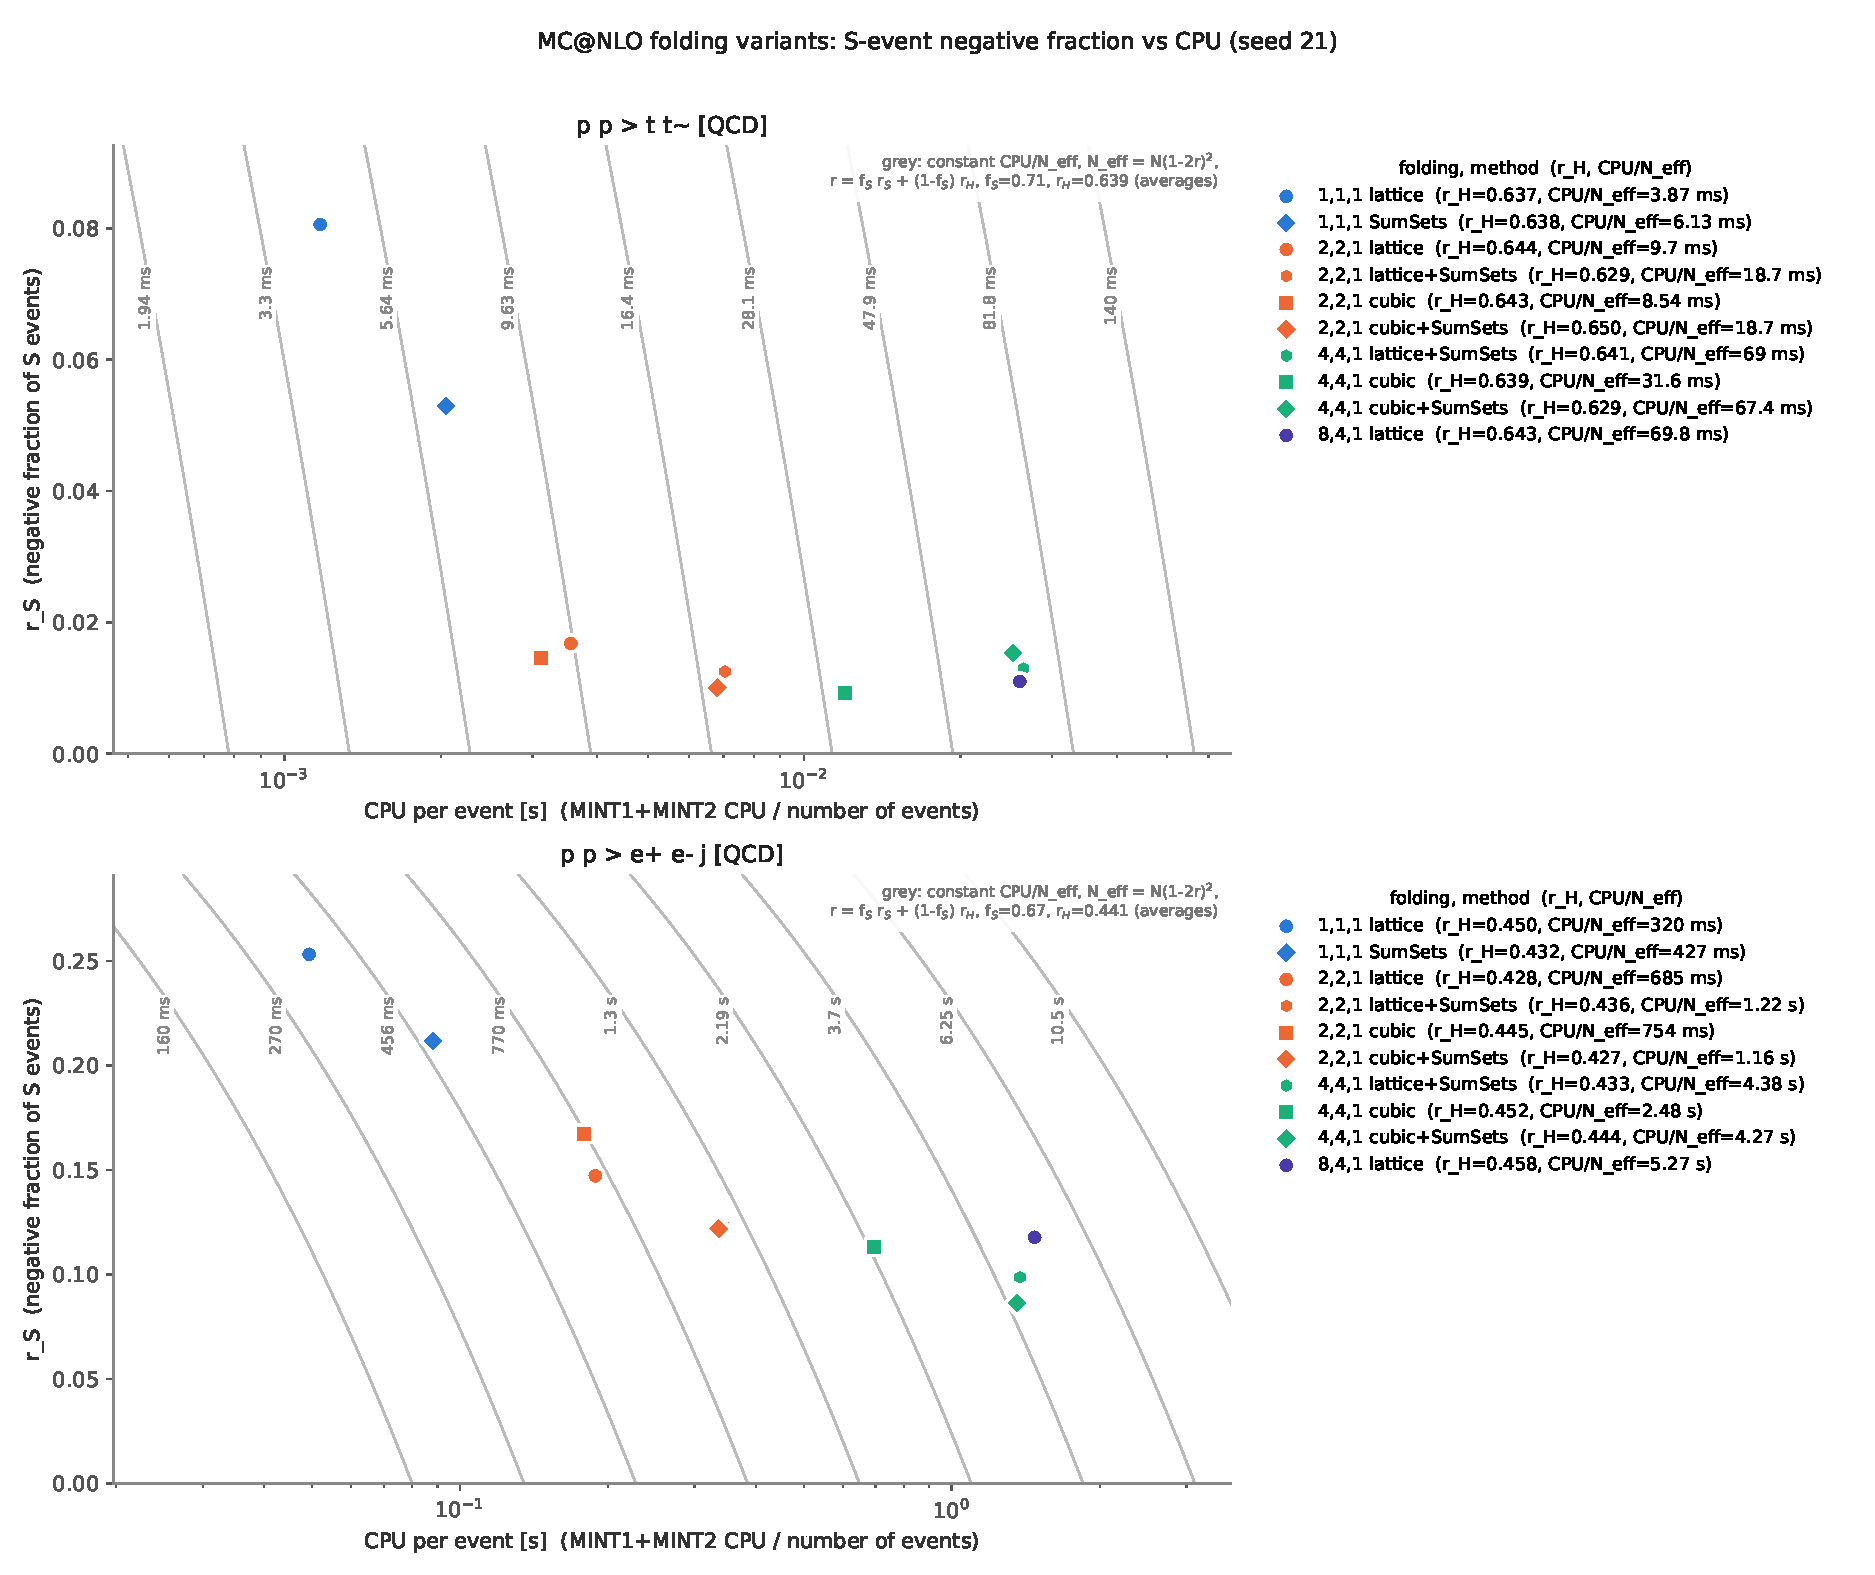
\includegraphics[width=0.92\textwidth]{rS_vs_cpu.pdf}
\caption{$\rS$ versus CPU per event for $pp\to t\bar t$ (top) and $pp\to e^+e^-j$ (bottom).
Grey lines: constant CPU$/\Neff$. Colour: folding; shape: method.}
\label{fig:tt_eej}
\end{figure}

\begin{figure}[p]
\centering
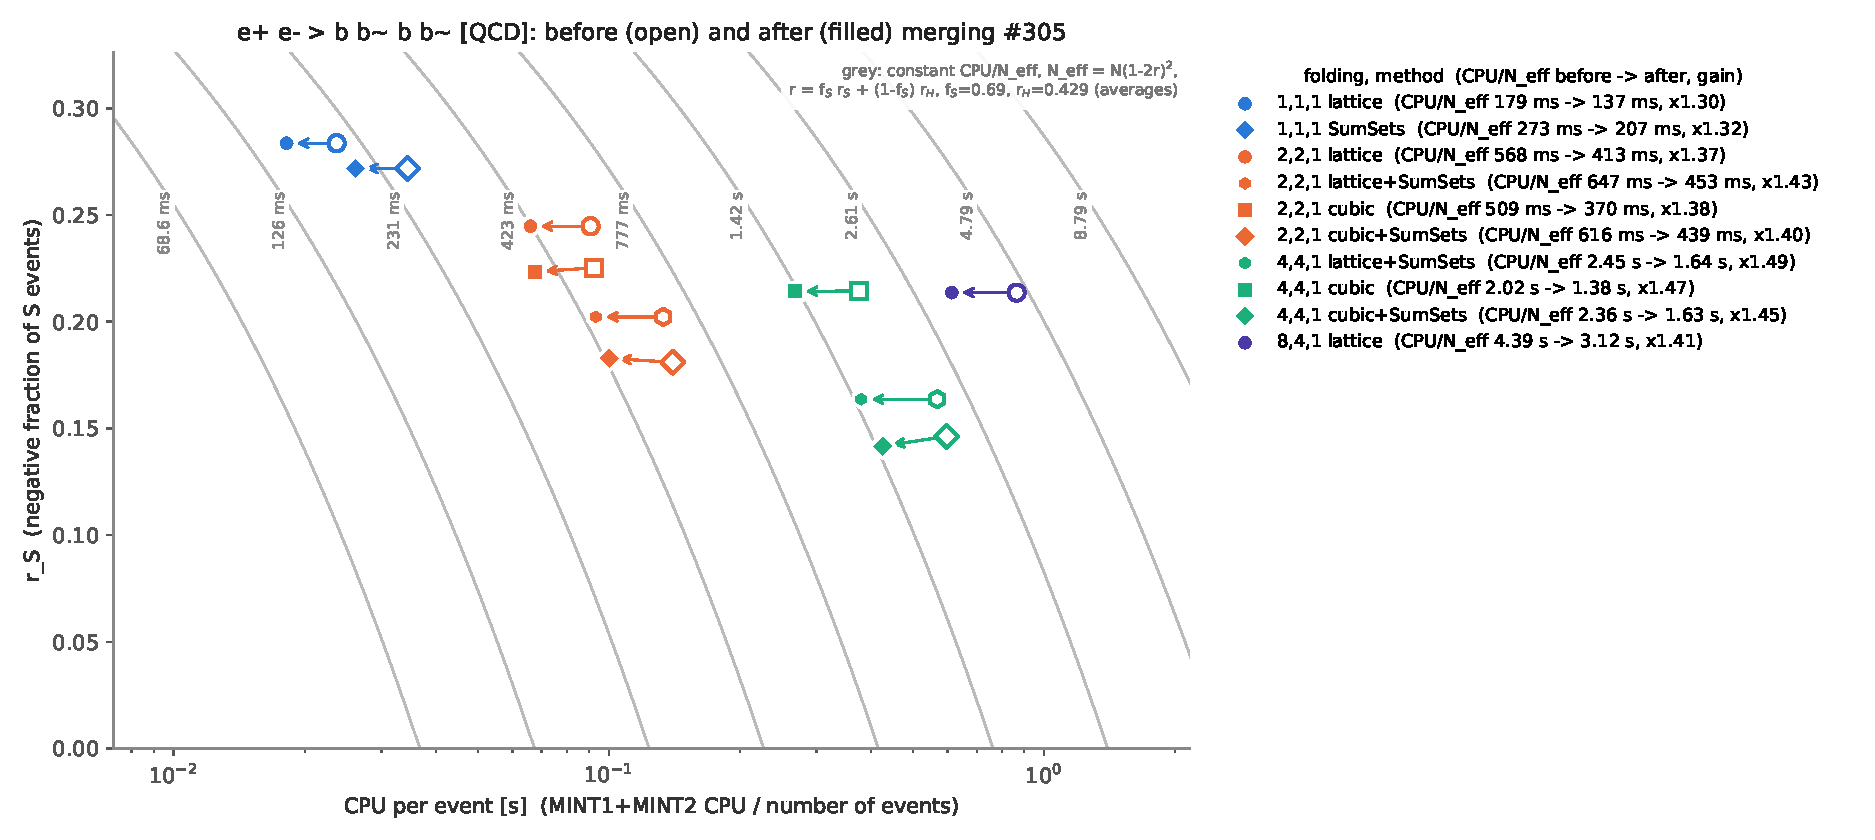
\includegraphics[width=0.92\textwidth]{rS_vs_cpu_ee4b_305_shift.pdf}
\caption{$e^+e^-\to b\bar b b\bar b$: shift of each variant when the cached-Born
optimisations of PR~\#305 are added (open: before, filled: after; same machine load).}
\label{fig:ee4b}
\end{figure}

\begin{figure}[p]
\centering
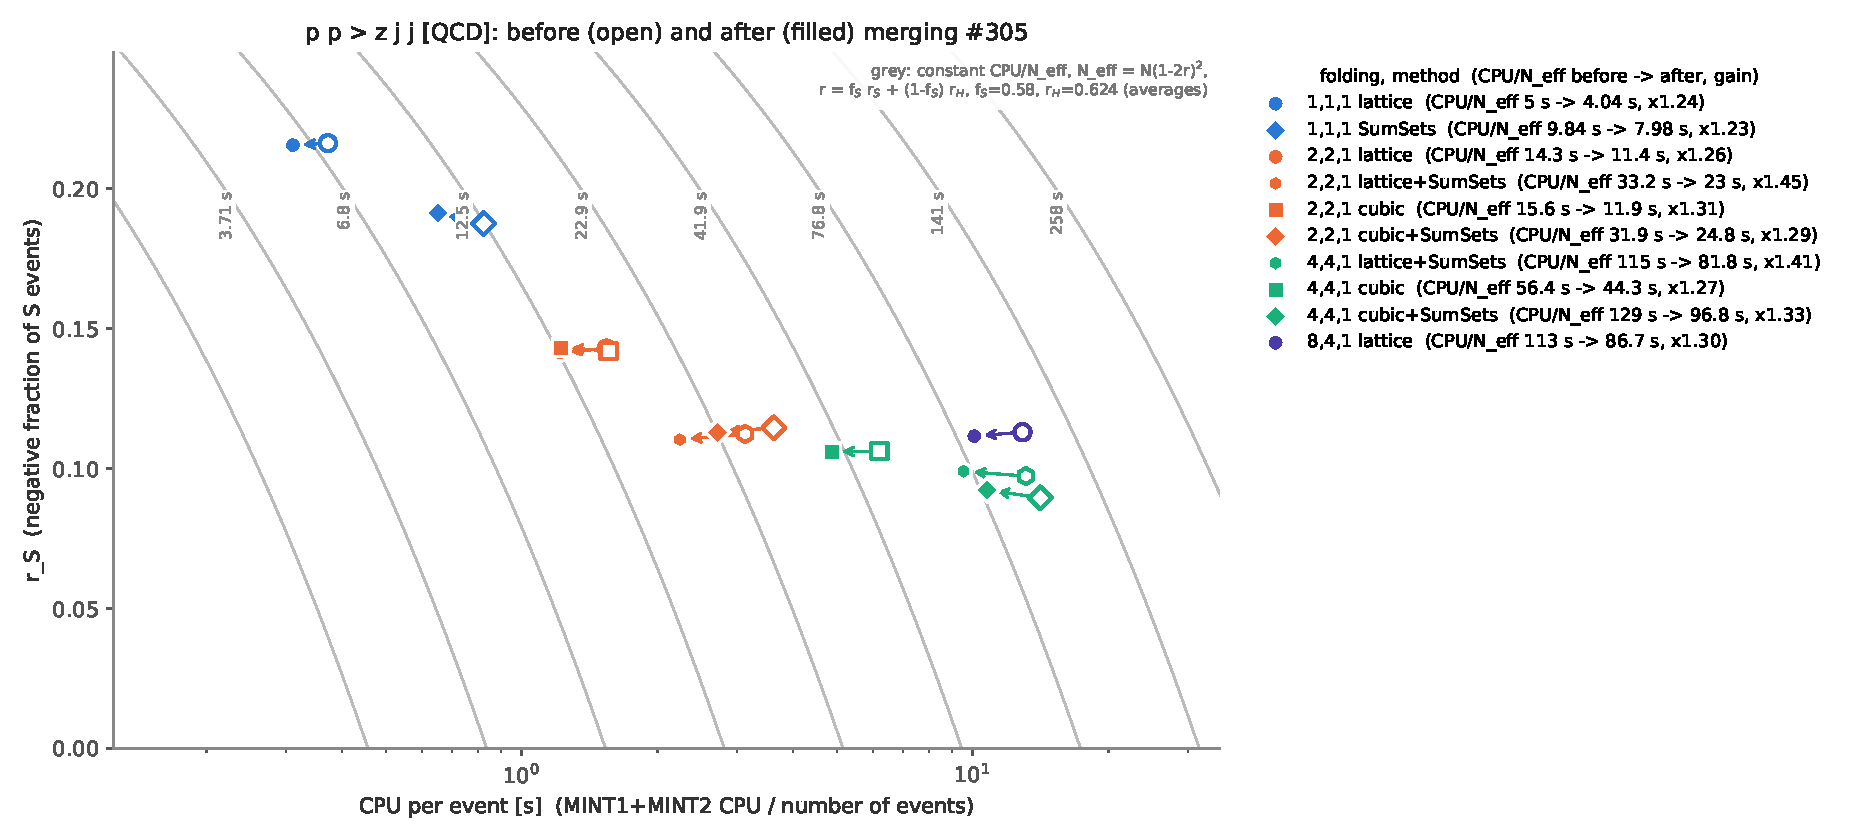
\includegraphics[width=0.92\textwidth]{rS_vs_cpu_zjj_305_shift.pdf}
\caption{$pp\to Zjj$: as figure~\ref{fig:ee4b}.}
\label{fig:zjj}
\end{figure}

\subsection{Comments}

\paragraph{Today's folding against the new modes.}
Table~\ref{tab:summary} compares the old $8\times4\times1$ folding with $2\times2\times1$
using the cubic map and the sum over sets. The new combination reaches the same total
negative fraction, or a lower one, at 3.5 to 7 times less CPU per effective event. Most of
the gain over the old $2\times2\times1$ lattice comes from summing the sets; the cubic map
adds a smaller, process-dependent improvement.

\begin{table}[t]
\centering
\begin{tabular}{lcccc}
\toprule
process & \multicolumn{2}{c}{8,4,1 lattice} & \multicolumn{2}{c}{2,2,1 cubic + sum}\\
 & $r$ & CPU$/\Neff$ & $r$ & CPU$/\Neff$\\
\midrule
$pp\to t\bar t$ & 0.195 & 69.8 ms & 0.198 & 18.7 ms\\
$pp\to e^+e^-j$ & 0.236 & 5.27 s & 0.231 & 1.16 s\\
$e^+e^-\to b\bar b b\bar b$ (with \#305) & 0.278 & 3.12 s & 0.261 & 0.44 s\\
$pp\to Zjj$ (with \#305) & 0.330 & 86.7 s & 0.335 & 24.8 s\\
\bottomrule
\end{tabular}
\caption{Today's $8\times4\times1$ folding against $2\times2\times1$ with the cubic map and the sum over FKS sets.}
\label{tab:summary}
\end{table}

\paragraph{Cubic map against lattice.}
At equal folding the two cost the same: the same number of points and images, as
figures~\ref{fig:ee4b} and~\ref{fig:zjj} show. The cubic map lowers $\rS$ in every pair for
$e^+e^-\to b\bar b b\bar b$ ($0.245\to0.223$, $0.202\to0.183$ with summed sets) and slightly
for $t\bar t$. For $e^+e^-j$ it is neutral with summed sets ($0.123$ against $0.122$) and worse without
($0.147$ against $0.167$ at $2\times2\times1$). It is better at $4\times4\times1$. For $Zjj$ it
is neutral at $2\times2\times1$. This matches section~\ref{sec:cubic}: the integrand has
steps, and with two images per variable the map can at best change the constant.

\paragraph{Summing over FKS sets.}
Summing always lowers $\rS$, as it must (section~\ref{sec:sumsets}): by 0.02 to 0.05. It
costs about twice the CPU per event, since the S part is evaluated for 3 to 4 sets per image.
Whether it pays in CPU$/\Neff$ depends on the weight of the S events in $r$:
\begin{itemize}
\item For $e^+e^-\to b\bar b b\bar b$ (S events 69\% of all events) it is the winning
ingredient.
\item For $Zjj$, $\rH\simeq0.62$ and the S events are only 58\% of the events. Lowering
$\rS$ from 0.142 to 0.110 hardly changes $r$. There, $2\times2\times1$ without summing is
the cheapest way to reach the plateau of $r\simeq0.33$.
\end{itemize}

\paragraph{The virt events.}
With the ``virt-trick'', the virtual correction enters the S events through its average
$A\,\mathcal B$. The residual $(V-A)\mathcal B$ is generated as separate ``virt'' events, a
fraction $\langle|V-A|\rangle/(\langle|S|\rangle+\langle|V-A|\rangle)$ of the events. Their sign is that of $V-A$, so about
half of them are negative, and no folding mode changes them. Because the folded S weights
become smaller in absolute value, the share of virt events grows with folding. They are
counted among the S events in our tables and set a floor $\simeq N_{\mathrm{virt}}/(2N_{\mathrm S})$
on $\rS$ (table~\ref{tab:floor}).

\paragraph{The H-event floor.}
In every process $\rH$ is independent of the folding mode, within statistics. It is $0.64$
for $t\bar t$, about $0.43$ for $e^+e^-j$ and $e^+e^-\to b\bar b b\bar b$, and $0.62$ for $Zjj$.
Folding acts on S events only, so once $\rS$ is small the total negative fraction is
$r\simeq(1-f_{\mathrm S})\rH$, with $f_{\mathrm S}$ the fraction of S events. For $t\bar t$ this floor
($0.29\times0.64=0.19$) is reached already at $2\times2\times1$. Further progress requires
work on the H events, i.e.\ on $R-\mathrm{MC}$, not on the integral of the S counterterms.

\paragraph{CPU per effective event without folding.}
For all four processes the cheapest setting in CPU$/\Neff$ remains $1\times1\times1$. Folding
reduces the number of negative events per generated event, not the cost per effective
event of the generation alone. It pays off when each event is expensive downstream (parton
shower, hadronisation, detector simulation), which is the situation folding was designed
for. The comparisons above are at fixed $r$, and there the new modes are cheaper.

\paragraph{Effect of PR~\#305.}
Rescaling the cached Born when only $\alpha_s$ changes, and keeping it across folds,
makes every variant 1.2 to 1.5 times cheaper per effective event
(tables~\ref{tab:ee4b}, \ref{tab:zjj}). The gain is larger for folded and summed-set
variants, which evaluate the Born more often. The negative fractions do not move.

\subsection{Has the S-event floor been reached?}
\label{sec:floor}
To see whether more folding still lowers the S-event negative fraction, we ran
$8\times4\times1$ with the cubic map and the sum over sets, which are the defaults, after PR~\#305.
These runs were done on the cluster, with the same seed and number of events as the
corresponding $2\times2\times1$ and $4\times4\times1$ runs. Table~\ref{tab:floor} compares
$\rS$ for the three foldings. The CPU of these runs is not comparable with the desktop runs
and is not quoted.

For each run we also give, in parentheses, the expected contribution of the virt events,
$N_{\mathrm{virt}}/(2N_{\mathrm S})$. It assumes that half of them are negative, as for a residual
$V-A$ symmetric around zero; $N_{\mathrm{virt}}$ is taken from the generation log, since the
events themselves do not record whether they are virt events.

\begin{table}[h]
\centering\small
\resizebox{\textwidth}{!}{%
\begin{tabular}{lccccccc}
\toprule
 & \multicolumn{3}{c}{$\rS$ (virt-event part)} & & \multicolumn{3}{c}{$r$}\\
process & $2\times2\times1$ & $4\times4\times1$ & $8\times4\times1$ & $\rH$ & 2,2,1 & 4,4,1 & 8,4,1\\
\midrule
\csname @@input\endcsname floor_rows.txt
\bottomrule
\end{tabular}}
\caption{S-event negative fraction with the cubic map and the sum over FKS sets, for three
foldings. In parentheses: expected contribution of the virt events. $\rH$ and the total
$r$ are for the $8\times4\times1$ runs and for each folding respectively.}
\label{tab:floor}
\end{table}

The floor is reached in every process, at the latest at $4\times4\times1$:
\begin{itemize}
\item \textbf{$pp\to t\bar t$.} $\rS$ equals the virt-event contribution at every folding
($0.010$, $0.015$, $0.011$). All the negative S events are virt events, and the floor is
reached already at $2\times2\times1$. Folding cannot do more here; a better virtual
surrogate (the dipole fits of the virt-trick study) could.
\item \textbf{$pp\to e^+e^-j$.} $\rS$ goes from $0.122$ ($2\times2\times1$) to $0.086$
($4\times4\times1$) and $0.094\pm0.004$ ($8\times4\times1$). It stops at about $0.09$, of which
$0.02$ comes from virt events. The remaining $0.07$ is consistent with the floor of
about $0.03$--$0.07$ found at fixed Born points with 256 points (table~\ref{tab:dumpr}).
\item \textbf{$e^+e^-\to b\bar b b\bar b$.} $0.183$, $0.142$, then $0.150\pm0.005$: the floor is
at about $0.145$, of which about $0.06$ comes from the virt events, which here are 8\% of all
events.
\item \textbf{$pp\to Zjj$.} Running (result pending).

\end{itemize}
The part of the floor that is not due to virt events corresponds to Born points where the
radiation integral of the S terms is negative, or so steep near the dead zones and cuts
that no affordable number of points resolves its sign. In all four processes the total $r$
no longer moves between $4\times4\times1$ and $8\times4\times1$: beyond
$2\times2\times1$ or $4\times4\times1$, extra folding only costs CPU.


%======================================================================
\section{Conclusions}
\label{sec:concl}
\begin{enumerate}
\item \textbf{Today's folding is a randomly shifted equally spaced lattice}: a first-order
rule in each folded variable, exact on average.
\item \textbf{A deterministic Simpson rule is biased} by $\mathcal O(10\%)$ on the average S
weight and cannot be used.
\item \textbf{The cubic map is a change of variables, not an interpolation}, so it works with
any number of images, including two. It is exact on average and turns the lattice into a
second-order rule. Its largest benefit is near the integrable soft and collinear endpoints,
where it improves the convergence from $n^{-1/2}$ to $n^{-1}$.
\item \textbf{Summing the S-event contributions over FKS sets removes a fluctuation that no
folding can touch}, and provably lowers $\rS$ at every Born point.
\item \textbf{With both options on and $2\times2\times1$ folding}, the negative fraction is as low as with today's
$8\times4\times1$, or lower, at 3.5 to 7 times less CPU per effective event, and the H events
then set the floor.
\end{enumerate}
Both options are on by default in \mg{} (\code{FoldCubic}, \code{FoldSumSets} in
\code{FKS\_params.dat}), together with the cached-Born optimisations of PR~\#305.

\begin{thebibliography}{99}
\bibitem{Frixione:2002ik}
S.~Frixione and B.~R.~Webber, \emph{Matching NLO QCD computations and parton shower
simulations}, JHEP \textbf{06} (2002) 029, [hep-ph/0204244].
\bibitem{Frixione:1995ms}
S.~Frixione, Z.~Kunszt and A.~Signer, \emph{Three jet cross-sections to next-to-leading
order}, Nucl.\ Phys.\ B \textbf{467} (1996) 399, [hep-ph/9512328].
\bibitem{Frederix:2009yq}
R.~Frederix, S.~Frixione, F.~Maltoni and T.~Stelzer, \emph{Automation of next-to-leading
order computations in QCD: the FKS subtraction}, JHEP \textbf{10} (2009) 003,
[arXiv:0908.4272].
\bibitem{Alwall:2014hca}
J.~Alwall et al., \emph{The automated computation of tree-level and next-to-leading order
differential cross sections, and their matching to parton shower simulations},
JHEP \textbf{07} (2014) 079, [arXiv:1405.0301].
\bibitem{Nason:2007vt}
P.~Nason, \emph{MINT: a computer program for adaptive Monte Carlo integration and generation
of unweighted distributions}, arXiv:0709.2085.
\bibitem{Cranley:1976}
R.~Cranley and T.~N.~L.~Patterson, \emph{Randomization of number theoretic methods for
multiple integration}, SIAM J.\ Numer.\ Anal.\ \textbf{13} (1976) 904.
\bibitem{Sidi:1993}
A.~Sidi, \emph{A new variable transformation for numerical integration}, in
\emph{Numerical Integration IV}, Birkh\"auser (1993) 359.
\bibitem{Valassi:2026pgd}
A.~Valassi, \emph{MadVfold}, arXiv:2609.23500.
\end{thebibliography}

\end{document}
